\chapter{Solução Desenvolvida}

\section{Visão Geral}

O projeto consistiu em uma plataforma de aprendizado de programação em Python, com foco em iniciantes. A plataforma é composta por um conjunto de quizzes, desafios e projetos, que são utilizados para fixar o conteúdo aprendido. A plataforma também conta com um sistema de pontuação, que é utilizado para incentivar os usuários a realizarem os quizzes, desafios e projetos, além de compartilharem seus projetos com outros usuários. A plataforma também conta com um sistema de ranking, que é utilizado para mostrar aos usuários o desempenho deles em relação aos outros usuários.

\section{Requisitos}

Os requisitos funcionais da plataforma foram definidos com base nos objetivos do projeto, que são: ensinar programação em Python para iniciantes, de forma lúdica e interativa. Sendo que foram priorizados os requisitos de RF01 a RF09 para a primeira versão da plataforma. Os requisitos da plataforma são:

\begin{itemize}
    \item RF01: Cadastro de usuários: o sistema deve permitir que os usuários se cadastrem na plataforma.
    \item RF02: Login de usuários: o sistema deve permitir que os usuários façam login na plataforma.
    \item RF03: Visualização de quizzes e desafios: o sistema deve permitir que os usuários visualizem quizzes e desafios.
    \item RF04: Realização de quizzes: o sistema deve permitir que os usuários realizem quizzes para fixar o conteúdo.
    \item RF05: Realização de desafios: o sistema deve permitir que os usuários realizem desafios para fixar o conteúdo.
    \item RF06: Criação de projetos: o sistema deve permitir que os usuários criem projetos em Python.
    \item RF07: Compartilhamento de projetos: o sistema deve permitir que os usuários compartilhem projetos através de links.
    \item RF08: Pontuação: o sistema deve permitir que os usuários acumulem pontos ao realizar quizzes, desafios, projetos e compartilhar projetos.
    \item RF09: Visualização da pontuação: o sistema deve permitir que os usuários visualizem sua pontuação.
    \item RF09: Visualização de ranking: o sistema deve permitir que os usuários visualizem o ranking de pontos.
    \item RF10: Visualização do histórico de pontuação: o sistema deve permitir que os usuários visualizem o histórico de pontuação.
    \item RF11: Visualização do perfil: o sistema deve permitir que os usuários visualizem seu perfil.
    \item RF12: Edição do perfil: o sistema deve permitir que os usuários editem seu perfil.
    \item RF13: Exclusão do perfil e dados: o sistema deve permitir que os usuários excluam seu perfil e dados.
\end{itemize}

\section{A Distribuição do Software}

Com o propósito de reduzir as dificuldades associadas com o preparo do ambiente de desenvolvimento, desejou-se que a ferramenta proposta possuísse o mínimo de dependências possível, e que fosse compatível com qualquer sistema operacional. Uma forma de se atingir este objetivo foi através do uso de uma solução que fosse executada à partir do navegador.

A distribuição padrão do Python, conhecida como CPython, é implementada em C, e não roda nativamente no navegador. Existem poucas soluções que viabilizem isso, sendo o WebAssembly a mais completa. Trata-se de um padrão que define um formato de código binário de baixo nível capaz de ser executado à partir de um navegador. É possível compilar o interpretador de Python para WebAssembly, tornando possível sua execução em ambiente Web.

No entanto, existem vários desafios de integração entre o código do interpretador e o ambiente do navegador, e por isso não basta uma simples recompilação. O projeto Pyodide não só prepara a compilação do interpretador do Python, como também tem uma série de funções para integrar melhor os dois ambientes e promover contexto compartilhado entre Python e JavaScript.

Buscou-se então uma biblioteca JavaScript capaz de desenhar em um canvas com HTML5. Dentre as opções, escolheu-se o PixiJS. O objetivo passou a ser invocar o PixiJS à partir de código Python, de modo que o estudante pudesse desenhar formas geométricas, linhas e vértices com linhas de código simples.

\section{Arquitetura}

A arquitetura do sistema é composta por três componentes principais: o servidor, o cliente e o banco de dados. O servidor é responsável por receber as requisições do cliente e enviar as respostas. O cliente é responsável por enviar as requisições ao servidor e receber as respostas. O banco de dados é responsável por armazenar os dados do sistema.

\subsection{Servidor}

O servidor é responsável por receber as requisições do cliente e enviar as respostas. O servidor é composto por um conjunto de módulos que são responsáveis por realizar as tarefas do sistema. Cada módulo é responsável por uma tarefa específica. Os pacotes utilizados no servidor são:

\begin{itemize}
    \item \textbf{URL Patterns}: são padrões de URLs utilizados pelo Django Rest Framework para identificar as requisições recebidas pelo servidor.
    \item \textbf{Views}: são funções que são executadas quando uma requisição é recebida pelo servidor. As views são responsáveis por realizar as tarefas do sistema.
    \item \textbf{Serializers}: são classes que são utilizadas para serializar e desserializar os dados recebidos e enviados pelo servidor. As classes de serialização são responsáveis por converter os dados recebidos e enviados pelo servidor para o formato JSON.
    \item \textbf{Models}: são classes que são utilizadas para representar os dados do sistema. As classes de modelo são responsáveis por representar os dados do sistema no banco de dados.
\end{itemize}

\begin{figure}[H]
    \centering
    \caption{Representação de pacotes e tecnologias do servidor}
    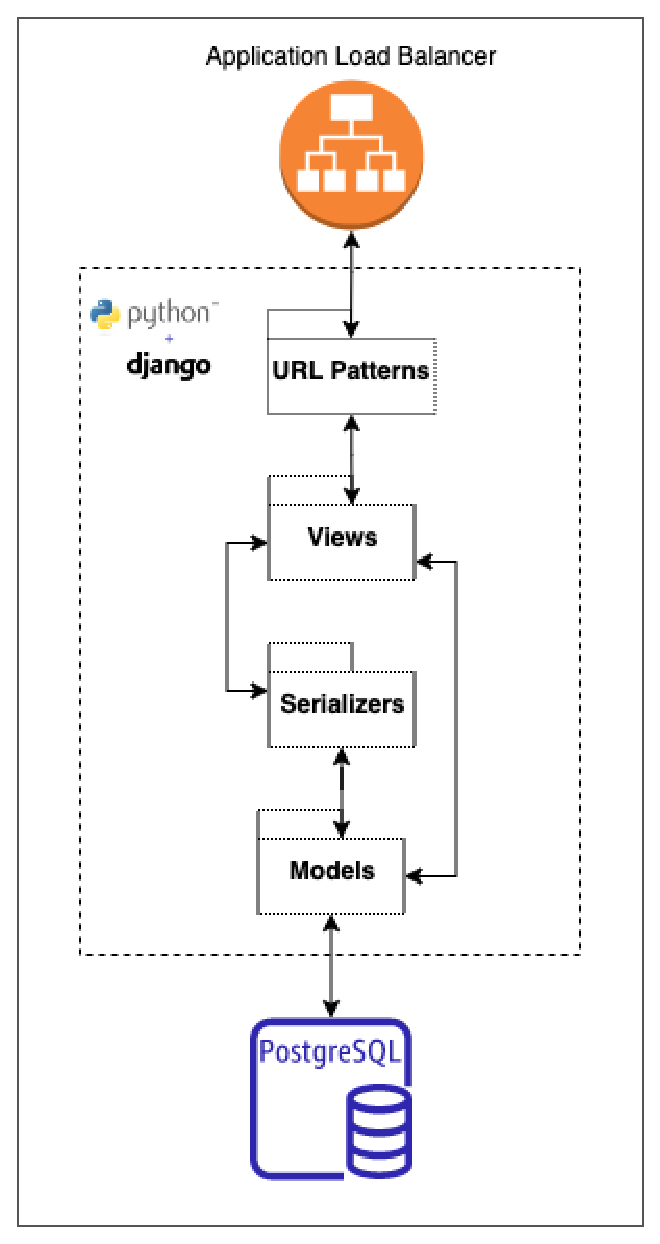
\includegraphics[keepaspectratio=true,scale=0.6]{figuras/backend_packages.eps}
    \legend{Fonte: Autores}
    \label{fig:backend_packages}
\end{figure}

\subsection{Cliente}

O cliente é responsável por enviar as requisições ao servidor e receber as respostas. O cliente é composto por um conjunto de módulos que são responsáveis por realizar as tarefas do sistema. Cada módulo é responsável por uma tarefa específica. Os pacotes utilizados no cliente são:

\begin{itemize}
    \item \textbf{Routers}: são classes que são utilizadas para definir as rotas da aplicação. Através das rotas é renderizado o componente correto para cada rota.
    \item \textbf{Components}: são classes que são utilizadas para definir os componentes da aplicação. Os componentes possuem uma estrutura HTML e são responsáveis por renderizar a interface do usuário.
    \item \textbf{Containers}: são classes que são utilizadas para definir os containers da aplicação. Os containers possuem a lógicas de negócio da aplicação.
    \item \textbf{Services}: são classes que são utilizadas para definir os serviços da aplicação. Os serviços são responsáveis por realizar as requisições ao servidor.
\end{itemize}

\begin{figure}[H]
    \centering
    \caption{Representação de pacotes e tecnologias do cliente}
    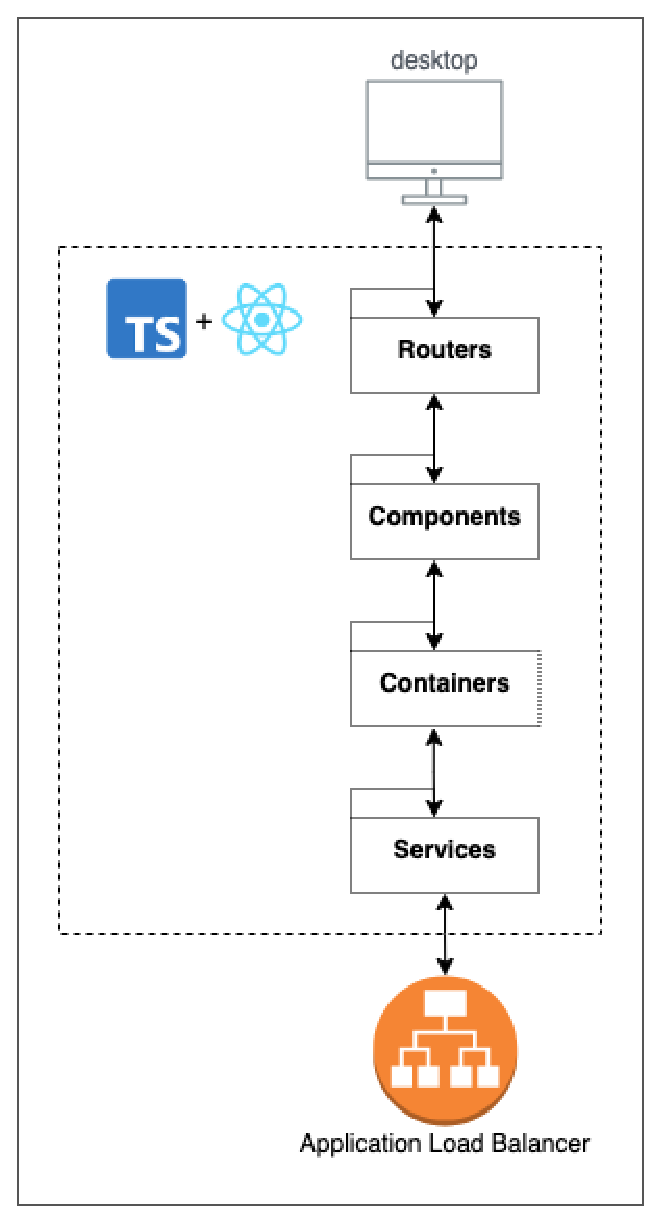
\includegraphics[keepaspectratio=true,scale=0.6]{figuras/frontend_packages.eps}
    \legend{Fonte: Autores}
    \label{fig:frontend_packages}
\end{figure}


\subsection{Modelo de Dados}

Um modelo de dados é uma representação abstrata de como os dados são estruturados e como eles se relacionam entre si. Ele é utilizado para descrever a estrutura lógica e conceitual dos dados, independentemente da forma como eles são armazenados ou implementados em um sistema. Existem vários tipos de modelos de dados, como o modelo relacional, o modelo de objeto-relacional e o modelo de dados NoSQL.

A escolha do modelo de dados é uma decisão importante, pois ela afeta diretamente a forma como os dados são armazenados e manipulados. O modelo de dados escolhido deve ser capaz de atender as necessidades do sistema. O modelo de dados escolhido para o sistema é o modelo relacional, pois ele é o modelo de dados mais utilizado no mundo e é capaz de atender as necessidades do sistema.

Abaixo é apresentado o modelo de dados do sistema. O modelo de dados é composto por 4 entidades: \textit{User}, \textit{Project}, \textit{Quizz} e \textit{Score}. Além das entidades, o modelo de dados é composto por 4 relacionamentos entre as entidades: \textit{SocialUser}, \textit{QuizzAnswer}, \textit{UserQuizzAnswer} e \textit{MonthlyScore}:

\begin{figure}[H]
    \centering
    \caption{Modelo de dados do sistema}
    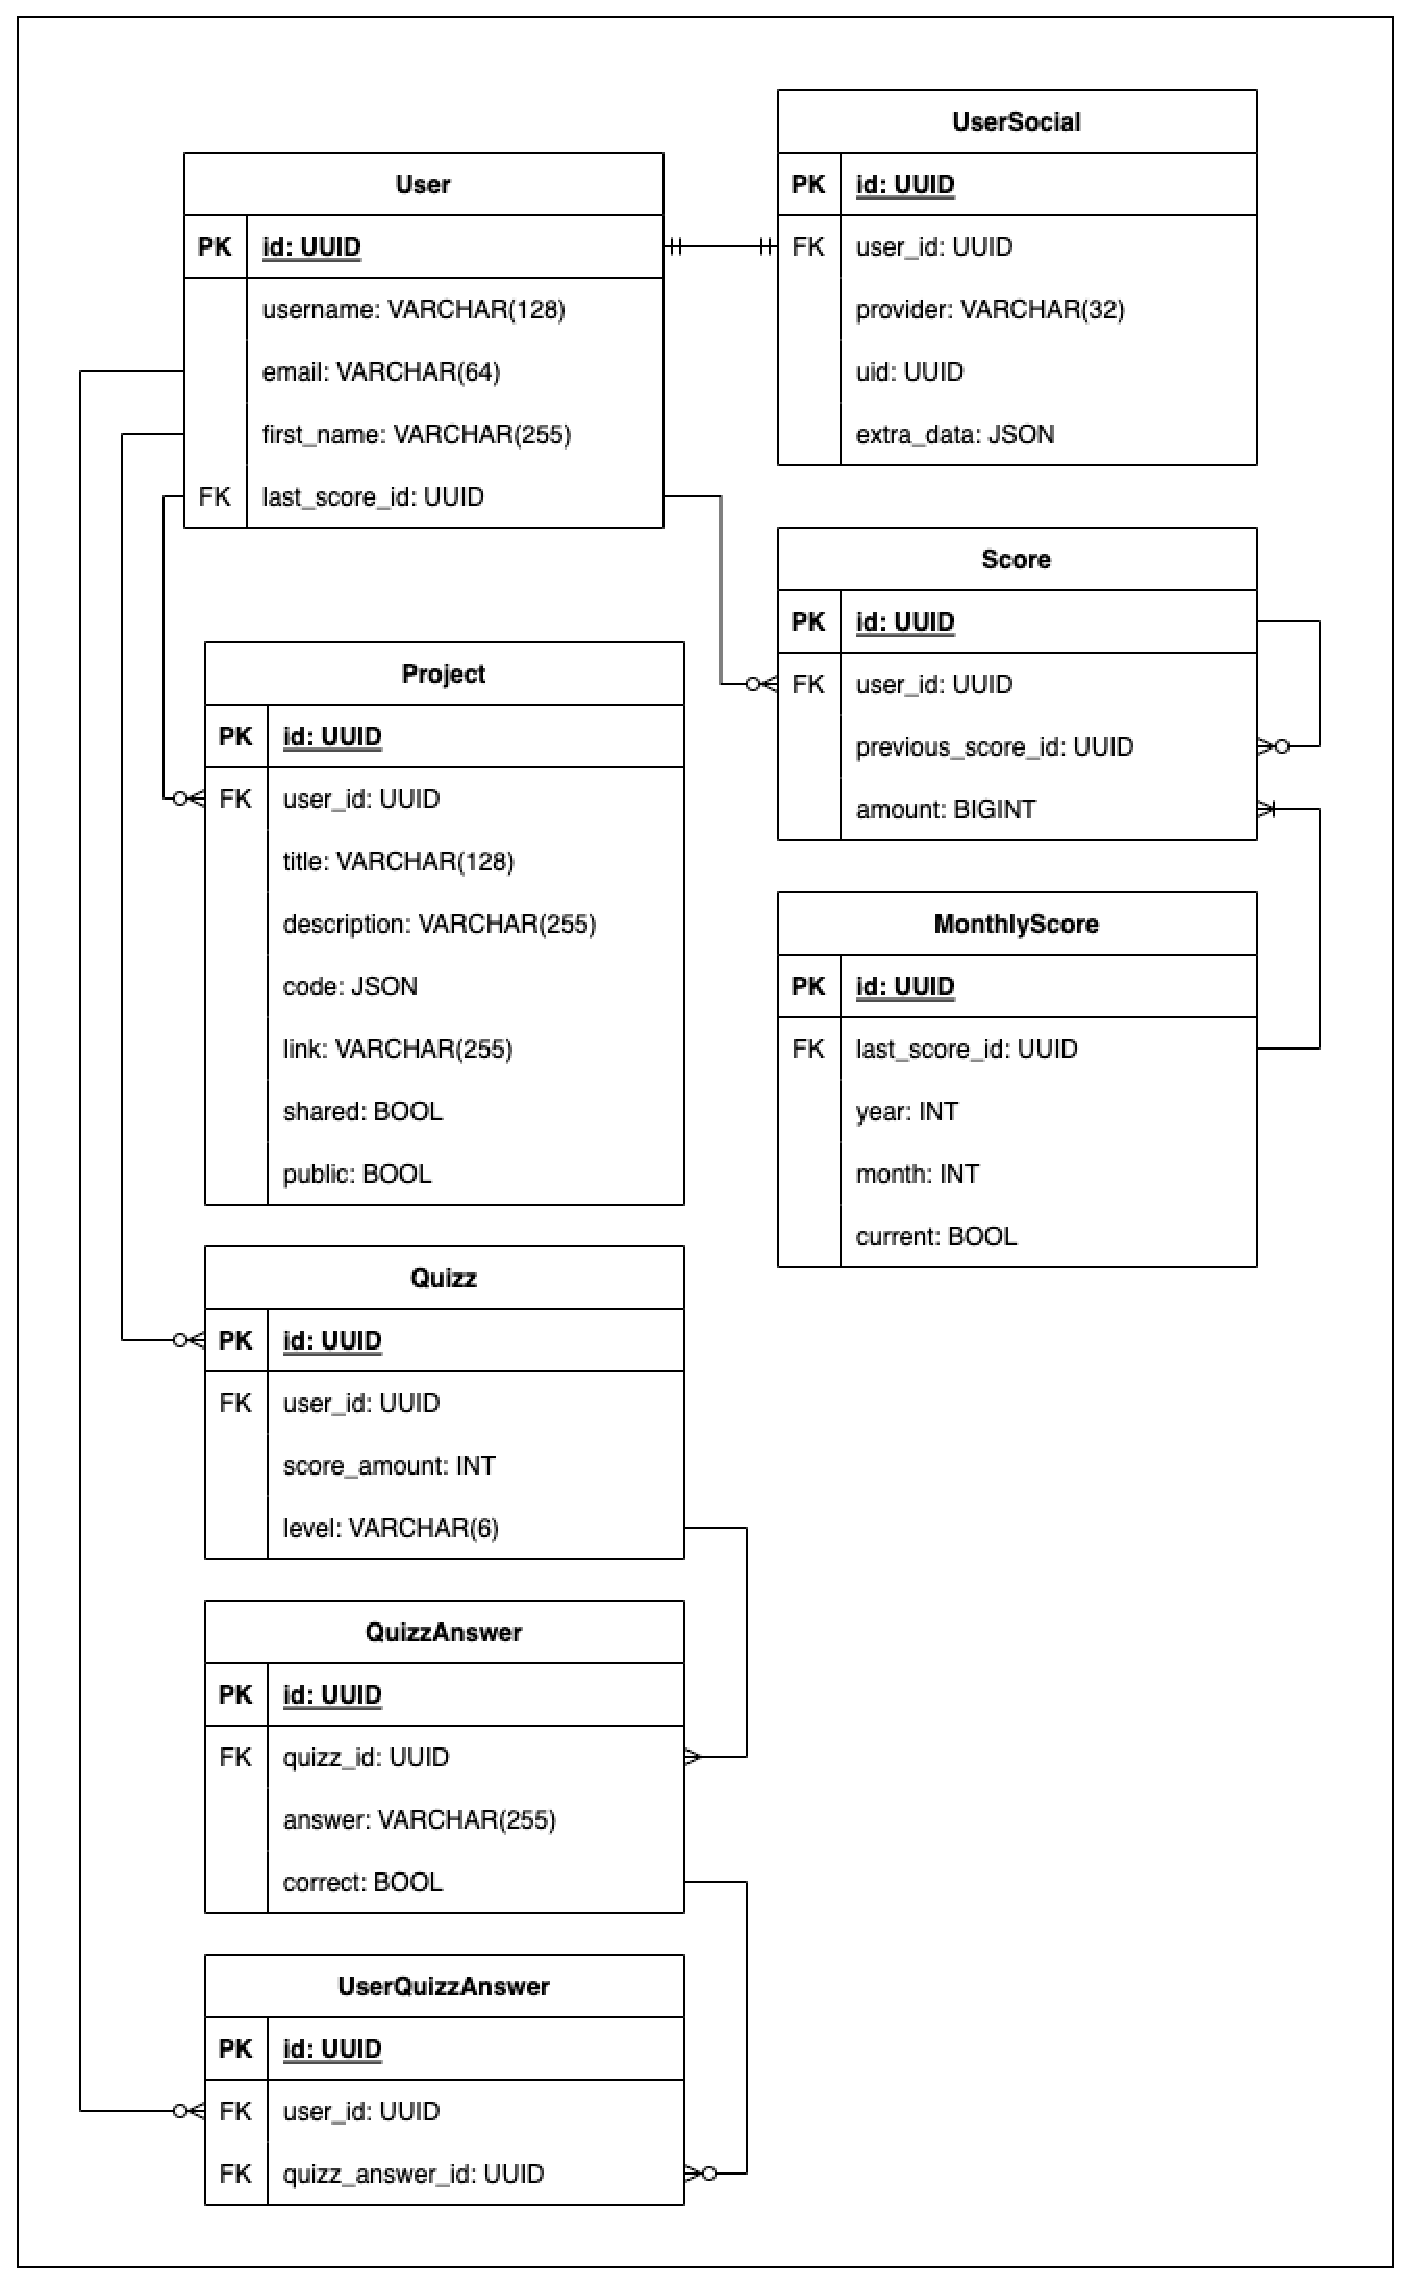
\includegraphics[keepaspectratio=true,scale=0.5]{figuras/modelo_de_dados.eps}
    \legend{Fonte: Autores}
    \label{fig:modelo_dados}
\end{figure}


\subsection{Configuração do Ambiente de Produção}

\subsubsection{Servidor}

O ambiente de produção do servidor é composto por um conjunto de ferramentas que são utilizadas para garantir a disponibilidade, escalabilidade, segurança e desempenho dos sistemas em execução. As ferramentas utilizadas no ambiente de produção do servidor são:

\begin{itemize} \label{itemize:server_production}
    \item \textbf{Python}: é uma linguagem de programação de alto nível, interpretada, de uso geral, criada por Guido van Rossum em 1989. Ela se destaca pela sua sintaxe clara e concisa, além de possuir uma grande variedade de bibliotecas e frameworks, tornando-a uma linguagem versátil e popular para desenvolvimento de diversas aplicações.
    \item \textbf{Django Rest Framework}: é um conjunto de ferramentas para criar aplicativos RESTful com o framework web Django. Ele fornece uma série de recursos para facilitar o desenvolvimento de APIs, como serialização automática de objetos do Django, autenticação, permissões, paginação e suporte a diferentes formatos de dados (JSON, XML, etc).
    \item \textbf{Docker}: é uma plataforma de software que permite aos desenvolvedores e administradores de sistemas embalar, distribuir e executar aplicativos em contêineres. Um contêiner é uma forma de isolamento de sistema, onde a aplicação e suas dependências são embaladas em um pacote, junto com tudo o que é necessário para rodá-lo, incluindo o sistema operacional, bibliotecas e configurações.
    \item \textbf{PostgreSQL}: é um sistema gerenciador de banco de dados relacional de código aberto. Ele é conhecido por sua robustez, escalabilidade e suporte a recursos avançados, como transações de nível de banco de dados, gatilhos, armazenamento de objetos, entre outros.
    \item \textbf{Route 53}: é um serviço de DNS gerenciado pela Amazon Web Services (AWS) que permite aos desenvolvedores criar domínios personalizados e hospedar sites na nuvem. Ele fornece alta disponibilidade e tolerância a falhas, além de suporte a várias regiões geográficas.
    \item \textbf{Elastic Load Balancing (ELB)}: é um serviço de balanceamento de carga gerenciado pela Amazon Web Services (AWS) que distribui o tráfego entrante em várias instâncias de aplicativos em execução em um ou mais servidores. Ele permite aos desenvolvedores escalar horizontalmente suas aplicações, garantindo alta disponibilidade e tolerância a falhas, sem precisar gerenciar manualmente as configurações de balanceamento de carga.
    \item \textbf{Amazon Elastic Container Service (ECS)}: é um serviço de nuvem gerenciado pela Amazon Web Services (AWS) que permite aos desenvolvedores executar e escalar aplicativos em contêineres. Ele fornece uma abstração para gerenciar e escalar clusters de contêineres, além de integração com outros serviços da AWS, como o Elastic Load Balancing (ELB) e o Elastic Block Store (EBS)
    \item \textbf{Amazon Elastic Container Registry (ECR)}: é um serviço de nuvem gerenciado pela Amazon Web Services (AWS) que permite aos desenvolvedores armazenar e gerenciar imagens de contêineres Docker. Ele fornece uma abstração para armazenar e gerenciar imagens de contêineres, além de integração com outros serviços da AWS, como o Amazon Elastic Container Service (ECS) e o Amazon Elastic Kubernetes Service (EKS).
    \item \textbf{Amazon Relational Database Service (RDS)}: é um serviço de nuvem gerenciado pela Amazon Web Services (AWS) que permite aos desenvolvedores executar e escalar bancos de dados relacionais em nuvem. Ele fornece uma abstração para gerenciar e escalar clusters de bancos de dados relacionais, além de integração com outros serviços da AWS, como o Elastic Load Balancing (ELB) e o Elastic Block Store (EBS).
    \item \textbf{Terraform}: é uma ferramenta de automação de infraestrutura como código (IaC) que permite aos desenvolvedores declarar a infraestrutura de seus sistemas em um arquivo de configuração e, em seguida, executar esse arquivo para provisionar e gerenciar a infraestrutura de seus sistemas na nuvem.
\end{itemize}

\subsubsection{Cliente}

O ambiente de produção do cliente é composto por um conjunto de ferramentas que são utilizadas para garantir a disponibilidade, escalabilidade, segurança, desempenho e compatibilidade com diferentes dispositivos e navegadores dos sistemas web em execução. As ferramentas utilizadas no ambiente de produção do cliente são:

\begin{itemize} \label{itemize:cliente_production}
    \item \textbf{JavaScript}: é uma linguagem de programação de alto nível, interpretada e de uso geral, que é principalmente utilizada para criar scripts para páginas da web e aplicativos web. Ele permite que os desenvolvedores adicionem interatividade e dinamicidade às páginas da web, tornando-as mais atraentes e intuitivas para os usuários.
    \item \textbf{ReactJS}: ReactJS é um biblioteca JavaScript open-source para construir interfaces de usuário (UI). Ele foi desenvolvido pelo Facebook e tem sido amplamente adotado por outras empresas e comunidades. Ele permite aos desenvolvedores criar componentes de UI reutilizáveis e gerenciar seu estado de forma eficiente. ReactJS utiliza uma abordagem de programação baseada em componentes, onde cada componente é responsável por renderizar uma parte específica da UI e pode ser facilmente combinado com outros componentes para construir interfaces complexas. Ele também tem uma funcionalidade chamada de ``Virtual DOM'', que otimiza o desempenho das atualizações na tela.
    \item \textbf{Material UI}: Material-UI é um framework de interface de usuário de código aberto para React que segue as diretrizes de design do Material Design, um conjunto de diretrizes de design criadas pelo Google. Ele fornece uma coleção de componentes prontos para uso, como botões, caixas de seleção, tabelas e formulários, além de fornecer suporte a temas personalizados e adaptabilidade a diferentes tamanhos de tela. Ele é projetado para ser fácil de usar e personalizar, e se integra facilmente com outras bibliotecas e frameworks.
    \item \textbf{Amplify Hosting}: é uma funcionalidade dentro do Amplify que permite aos desenvolvedores hospedar facilmente aplicativos web estáticos, como páginas SPA (Single Page Application), sites estáticos e landing pages. Ele oferece uma forma simples de configurar e gerenciar o armazenamento e a distribuição de arquivos estáticos, além de suportar recursos avançados como roteamento personalizado, suporte ao CloudFront e integração com o CloudFormation.
\end{itemize}

\subsection{Configuração do Ambiente de Desenvolvimento}

\subsubsection{Servidor}

O ambiente de desenvolvimento do servidor além de ser composto pelas ferramentas utilizadas no ambiente de produção \ref{itemize:server_production}, também inclui ferramentas adicionais para facilitar o processo de desenvolvimento, como ferramentas de gerenciamento de código-fonte, integração contínua, testes automatizados, depuração e monitoramento. Além disso, é comum que o ambiente de desenvolvimento seja configurado para simular o ambiente de produção o mais fielmente possível, de forma a permitir que os desenvolvedores testem o código com precisão antes de lançá-lo em produção. As ferramentas utilizadas no ambiente de desenvolvimento do servidor são apresentadas a seguir:

\begin{itemize}
    \item \textbf{Pylint}: é uma ferramenta de análise de código para a linguagem de programação Python. Ele verifica o código para seguir as boas práticas de estilo, detecta erros e problemas de qualidade, e gera relatórios sobre o desempenho do código. Ele pode ser integrado com diversas IDEs e ferramentas de gerenciamento de código-fonte, e é amplamente utilizado para melhorar a qualidade e a manutenibilidade do código.
    \item \textbf{Mypy}: é uma ferramenta de verificação de tipos para a linguagem Python. Ele verifica o código para garantir que os tipos sejam usados corretamente, detectando erros de tipo em tempo de desenvolvimento, antes que eles sejam executados. Ele pode ser usado como uma ferramenta de linha de comando ou integrado com outras ferramentas de desenvolvimento, como IDEs e sistemas de gerenciamento de código-fonte.
    \item \textbf{Black}: Black é uma ferramenta de formatação automática de código para Python. Ele segue as boas práticas de estilo recomendadas pela comunidade Python, e formata o código de acordo com essas regras, garantindo que o código seja consistente e fácil de ler. Ele pode ser integrado com ferramentas de gerenciamento de código-fonte, como o Git, e usado como parte do fluxo de trabalho de desenvolvimento para garantir que o código seja formatado corretamente antes de ser enviado para o repositório.
    \item \textbf{Pre-commit}: Pre-commit é uma ferramenta de gerenciamento de configurações de hooks de commit para várias ferramentas de desenvolvimento. Ele permite que os desenvolvedores configurem várias verificações, como testes automatizados, análise de código e formatação, para serem executadas antes de cada commit. Isso garante que o código enviado para o repositório esteja de acordo com as boas práticas e padrões estabelecidos, e evita problemas de qualidade e compatibilidade.
    \item \textbf{Docker Compose}: é uma ferramenta de linha de comando para definir e executar aplicativos multi-contêiner usando o Docker. Ele permite que os desenvolvedores escrevam uma configuração simples em um arquivo YAML, descrevendo os contêineres, volumes e redes necessários para o aplicativo. Com essa configuração, os desenvolvedores podem facilmente criar e gerenciar os contêineres e suas dependências em ambiente de desenvolvimento, teste ou produção.
    \item \textbf{GitHub}: é uma plataforma de hospedagem de código-fonte baseada na web que fornece controle de versão, gerenciamento de projetos e colaboração para desenvolvedores. Ele é baseado no sistema de controle de versão Git e permite que os desenvolvedores armazenem, compartilhem e colaborem em projetos de software usando o Git. Ele também fornece recursos adicionais, como gerenciamento de tarefas, relatórios de erros, documentação e integração com outras ferramentas de desenvolvimento.
    \item \textbf{GitHub Actions}: é uma funcionalidade do GitHub que permite que os desenvolvedores criem e gerenciem fluxos de trabalho automatizados diretamente no GitHub. Ele permite que os desenvolvedores automatizem tarefas como testes, implantações, construções e entregas de software, sem precisar deixar a plataforma do GitHub. Ele fornece uma ampla variedade de ações pré-construídas e integrações com outras ferramentas, além de suportar scripts personalizados. Isso permite que os desenvolvedores aumentem a eficiência e reduzam o tempo de entrega, além de monitorar e auditar facilmente os fluxos de trabalho.
    \item \textbf{SonarCloud}: SonarCloud é uma plataforma de análise de código baseada na nuvem que fornece ferramentas de análise de qualidade de código, métricas e relatórios para desenvolvedores. Ele é projetado para ajudar os desenvolvedores a melhorar a qualidade, manutenibilidade e segurança do código. Ele suporta uma variedade de linguagens de programação, incluindo Java, C\#, JavaScript, TypeScript, Python, entre outras. Ele permite que os desenvolvedores façam análise estática de código, análise de segurança, monitoramento de cobertura de testes e outras verificações de qualidade.
\end{itemize}

\subsubsection{Cliente}

O ambiente de desenvolvimento do cliente além de ser composto pelas ferramentas utilizadas no ambiente de produção \ref{itemize:cliente_production}, também inclui ferramentas adicionais para facilitar o processo de desenvolvimento. As ferramentas utilizadas no ambiente de desenvolvimento do servidor são apresentadas a seguir:

\begin{itemize}
    \item \textbf{TypeScript}: é uma linguagem de programação de código aberto desenvolvida e mantida pela Microsoft. Ele é uma super set do javascript, isso significa que todo o código javascript é válido em TypeScript. Ele adiciona tipagem estática ao javascript, o que permite aos desenvolvedores escrever código mais confiável e fácil de manter, além de oferecer recursos avançados como inferência de tipos, classes, interfaces, além de suporte a orientação a objetos. TypeScript compila para javascript, o que significa que pode ser executado em qualquer lugar onde javascript é suportado.
    \item \textbf{ESLint}: é uma ferramenta de análise de código estática para JavaScript e outras linguagens baseadas em JavaScript, como JSX, TypeScript. Ele ajuda a identificar e corrigir problemas de qualidade de código, como erros de sintaxe, padrões de codificação não seguidos, e boas práticas de desenvolvimento.
    \item \textbf{Prettier}: é uma ferramenta de formatação de código para JavaScript e outras linguagens baseadas em JavaScript, como JSX, TypeScript. Ele segue uma série de regras de formatação predefinidas para garantir que o código seja consistente e fácil de ler.
    \item \textbf{Husky}: é uma ferramenta de gerenciamento de ganchos de commit para Git. Ele permite que os desenvolvedores configurem scripts para serem executados automaticamente antes de cada commit, teste, push e outras operações do Git. Ele é especialmente útil para automatizar tarefas como testes automatizados, análise de código e formatação, garantindo que o código enviado para o repositório esteja de acordo com as boas práticas e padrões estabelecidos.
    \item \textbf{ViteJS}: ViteJS é uma ferramenta de desenvolvimento web de código aberto que foi projetada para ser rápida e fácil de usar. Ele é um servidor de desenvolvimento baseado em JavaScript que permite aos desenvolvedores iniciar rapidamente projetos e experimentar novas ideias sem a necessidade de configuração complexa. Ele usa o recurso ES modules nativo do navegador para carregar módulos, o que permite aos desenvolvedores desfrutar de carregamento de módulos instantâneo sem a necessidade de configurar um transpilador como o Babel ou o Webpack. ViteJS também inclui recursos como live-reloading, suporte a TypeScript e JSX, e suporte a plugins. Ele é projetado para trabalhar especialmente bem com frameworks modernos como React, Vue e Svelte.
    \item \textbf{Yarn}: é um gerenciador de pacotes para JavaScript, similar ao npm (o gerenciador de pacotes padrão para Node.js), mas com algumas funcionalidades adicionais. Ele permite que os desenvolvedores instalem e gerenciem pacotes JavaScript e suas dependências de forma eficiente e segura. Ele oferece uma série de recursos adicionais, como gerenciamento de cache, garantia de reproducibilidade, e melhorias de desempenho no gerenciamento de dependências.
\end{itemize}

\section{A Ferramenta}

A ferramenta apresentada por este trabalho chama-se Enpyre, uma plataforma de aprendizado de programação focada exclusivamente na linguagem Python, que oferece uma abordagem baseada em jogos para o ensino de programação. A ferramenta permite aos usuários criar jogos de forma fácil e intuitiva, utilizando uma interface gráfica e um editor de texto para escrever código Python. Além disso, a ferramenta utiliza a biblioteca PixiJS para fornecer uma interface gráfica para os jogos criados.

\subsection{Disponibilidade}

A ferramenta está disponível em: https://enpyre-play.vercel.app/.

O repositório do trabalho está disponível em: https://github.com/Enpyre.

\subsection{Tela de boas-vindas}

\begin{figure}[H]
    \centering
    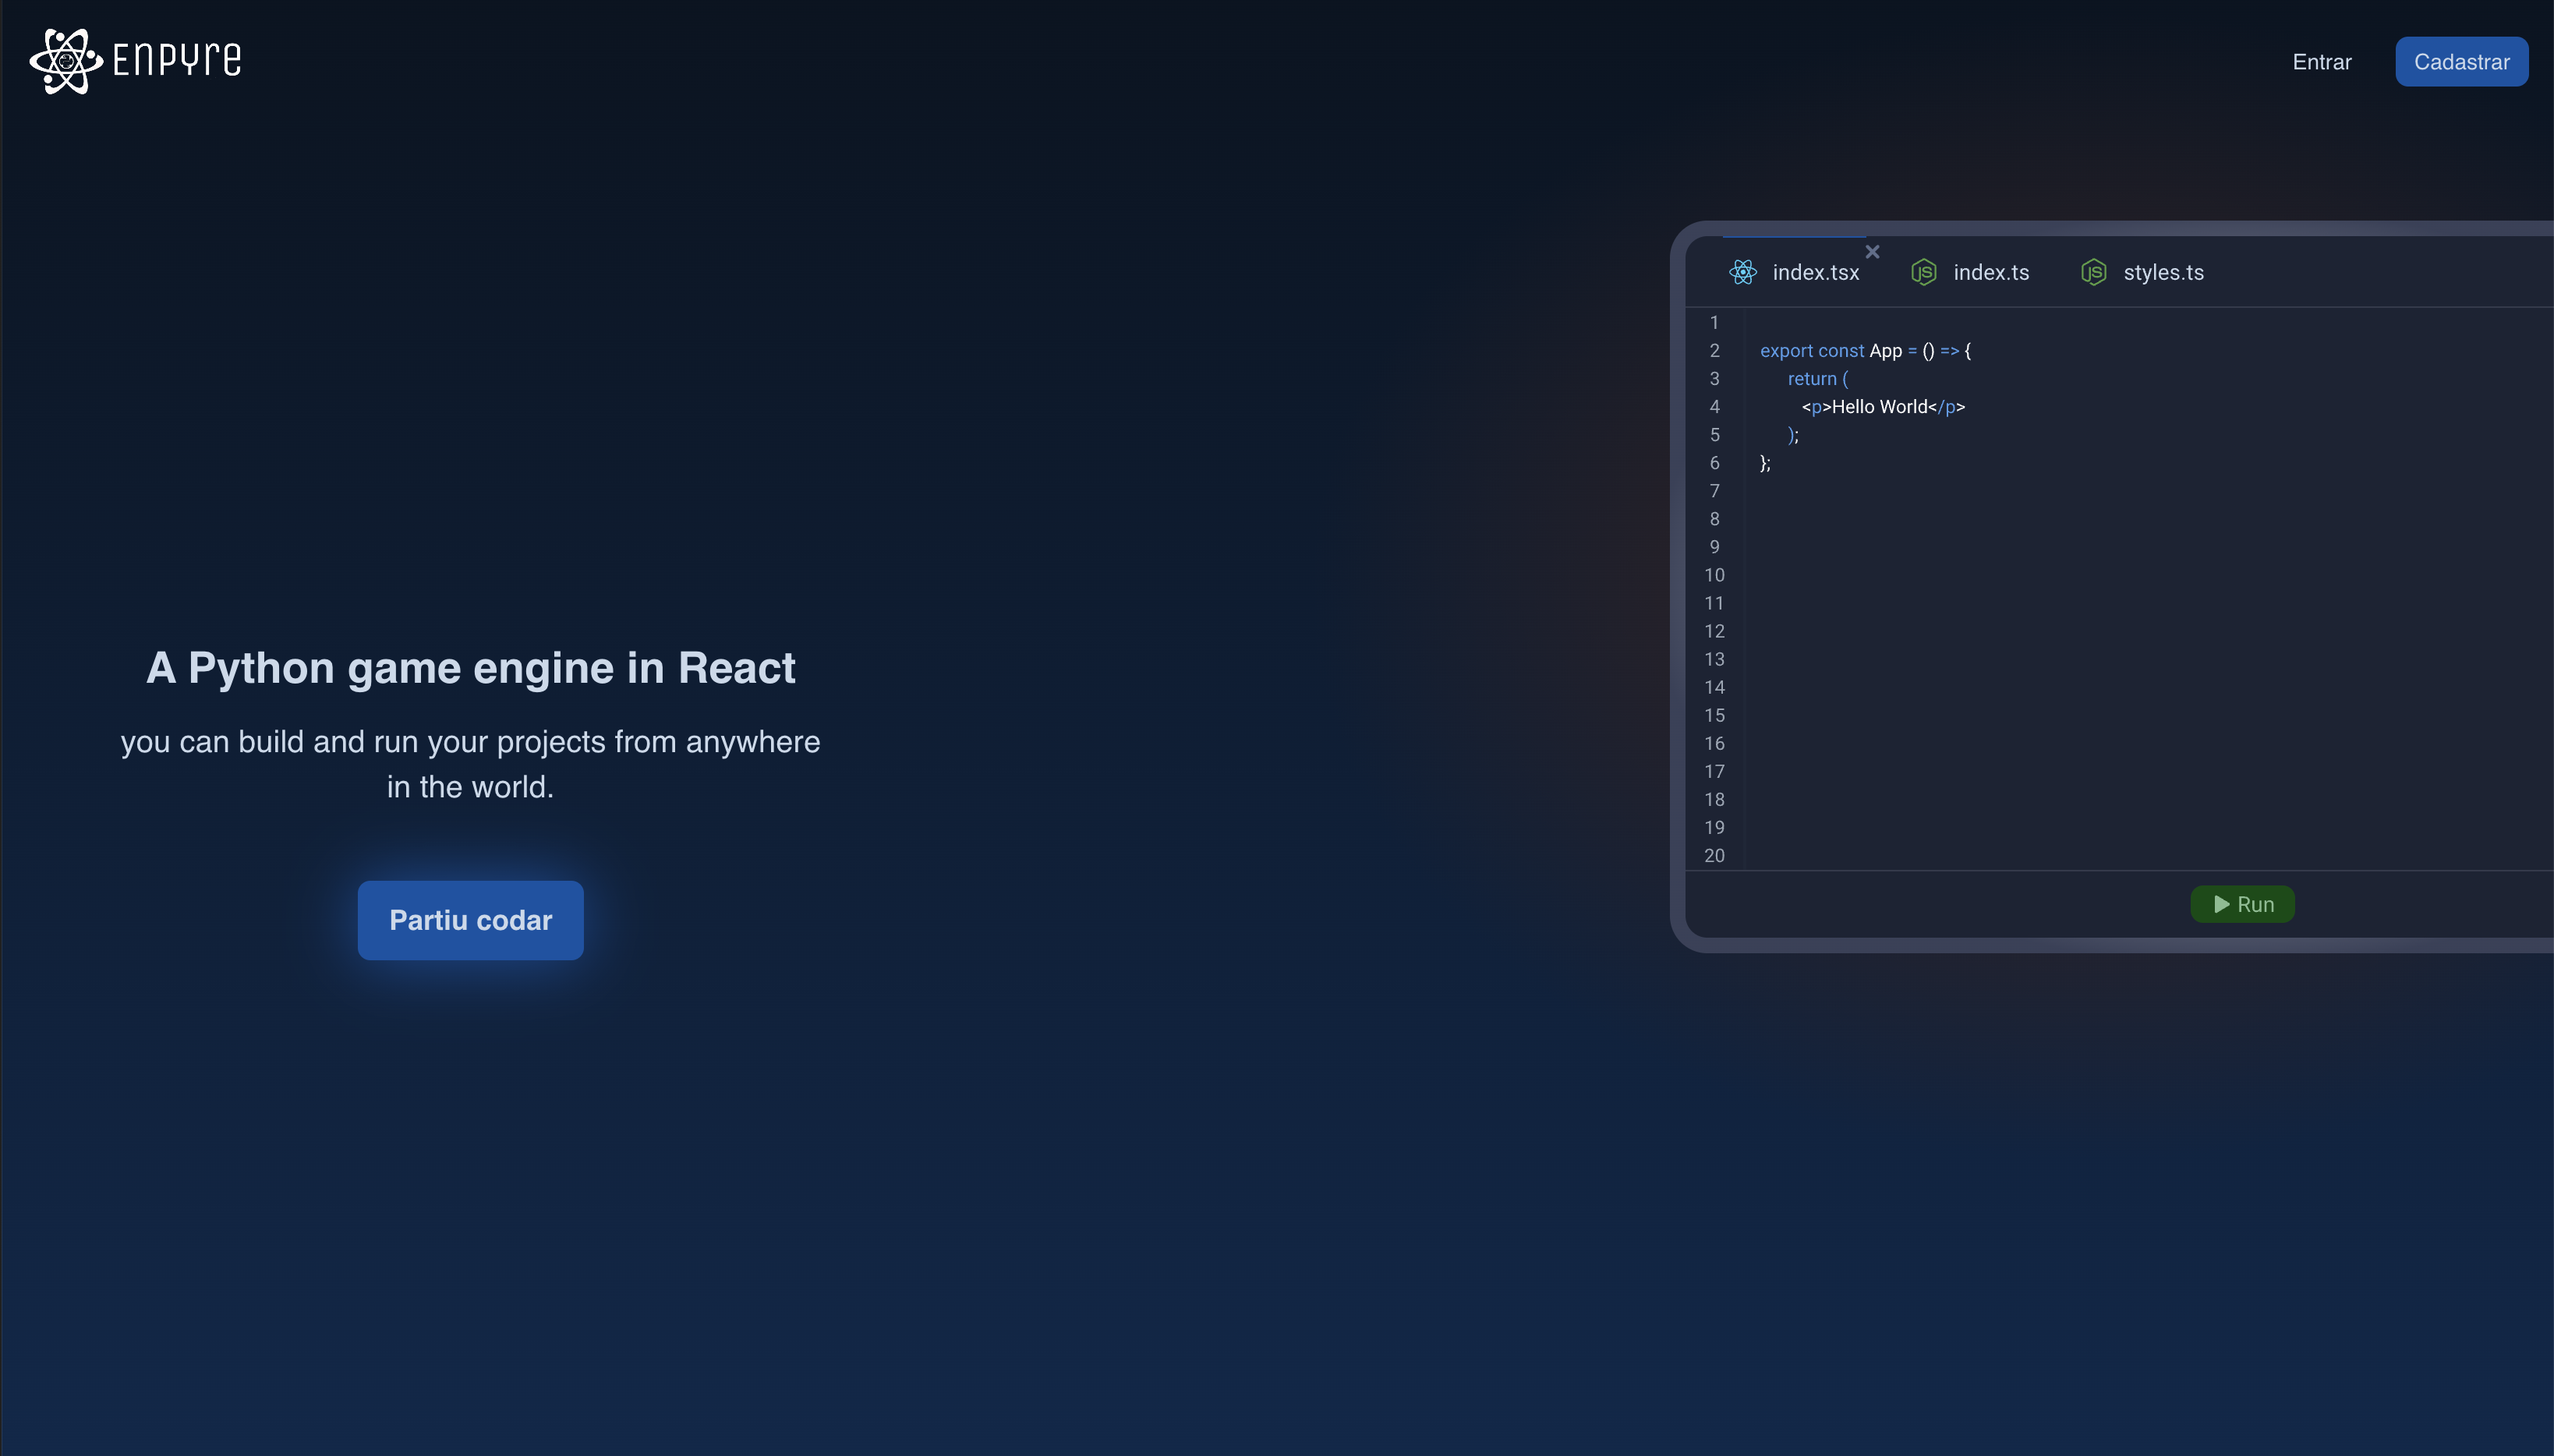
\includegraphics[width=0.8\textwidth]{figuras/boas-vindas.eps}
    \caption{Tela de boas-vindas}
    \label{fig:boas-vindas}
\end{figure}

\subsection{Tela de lista projetos}

\begin{figure}[H]
    \centering
    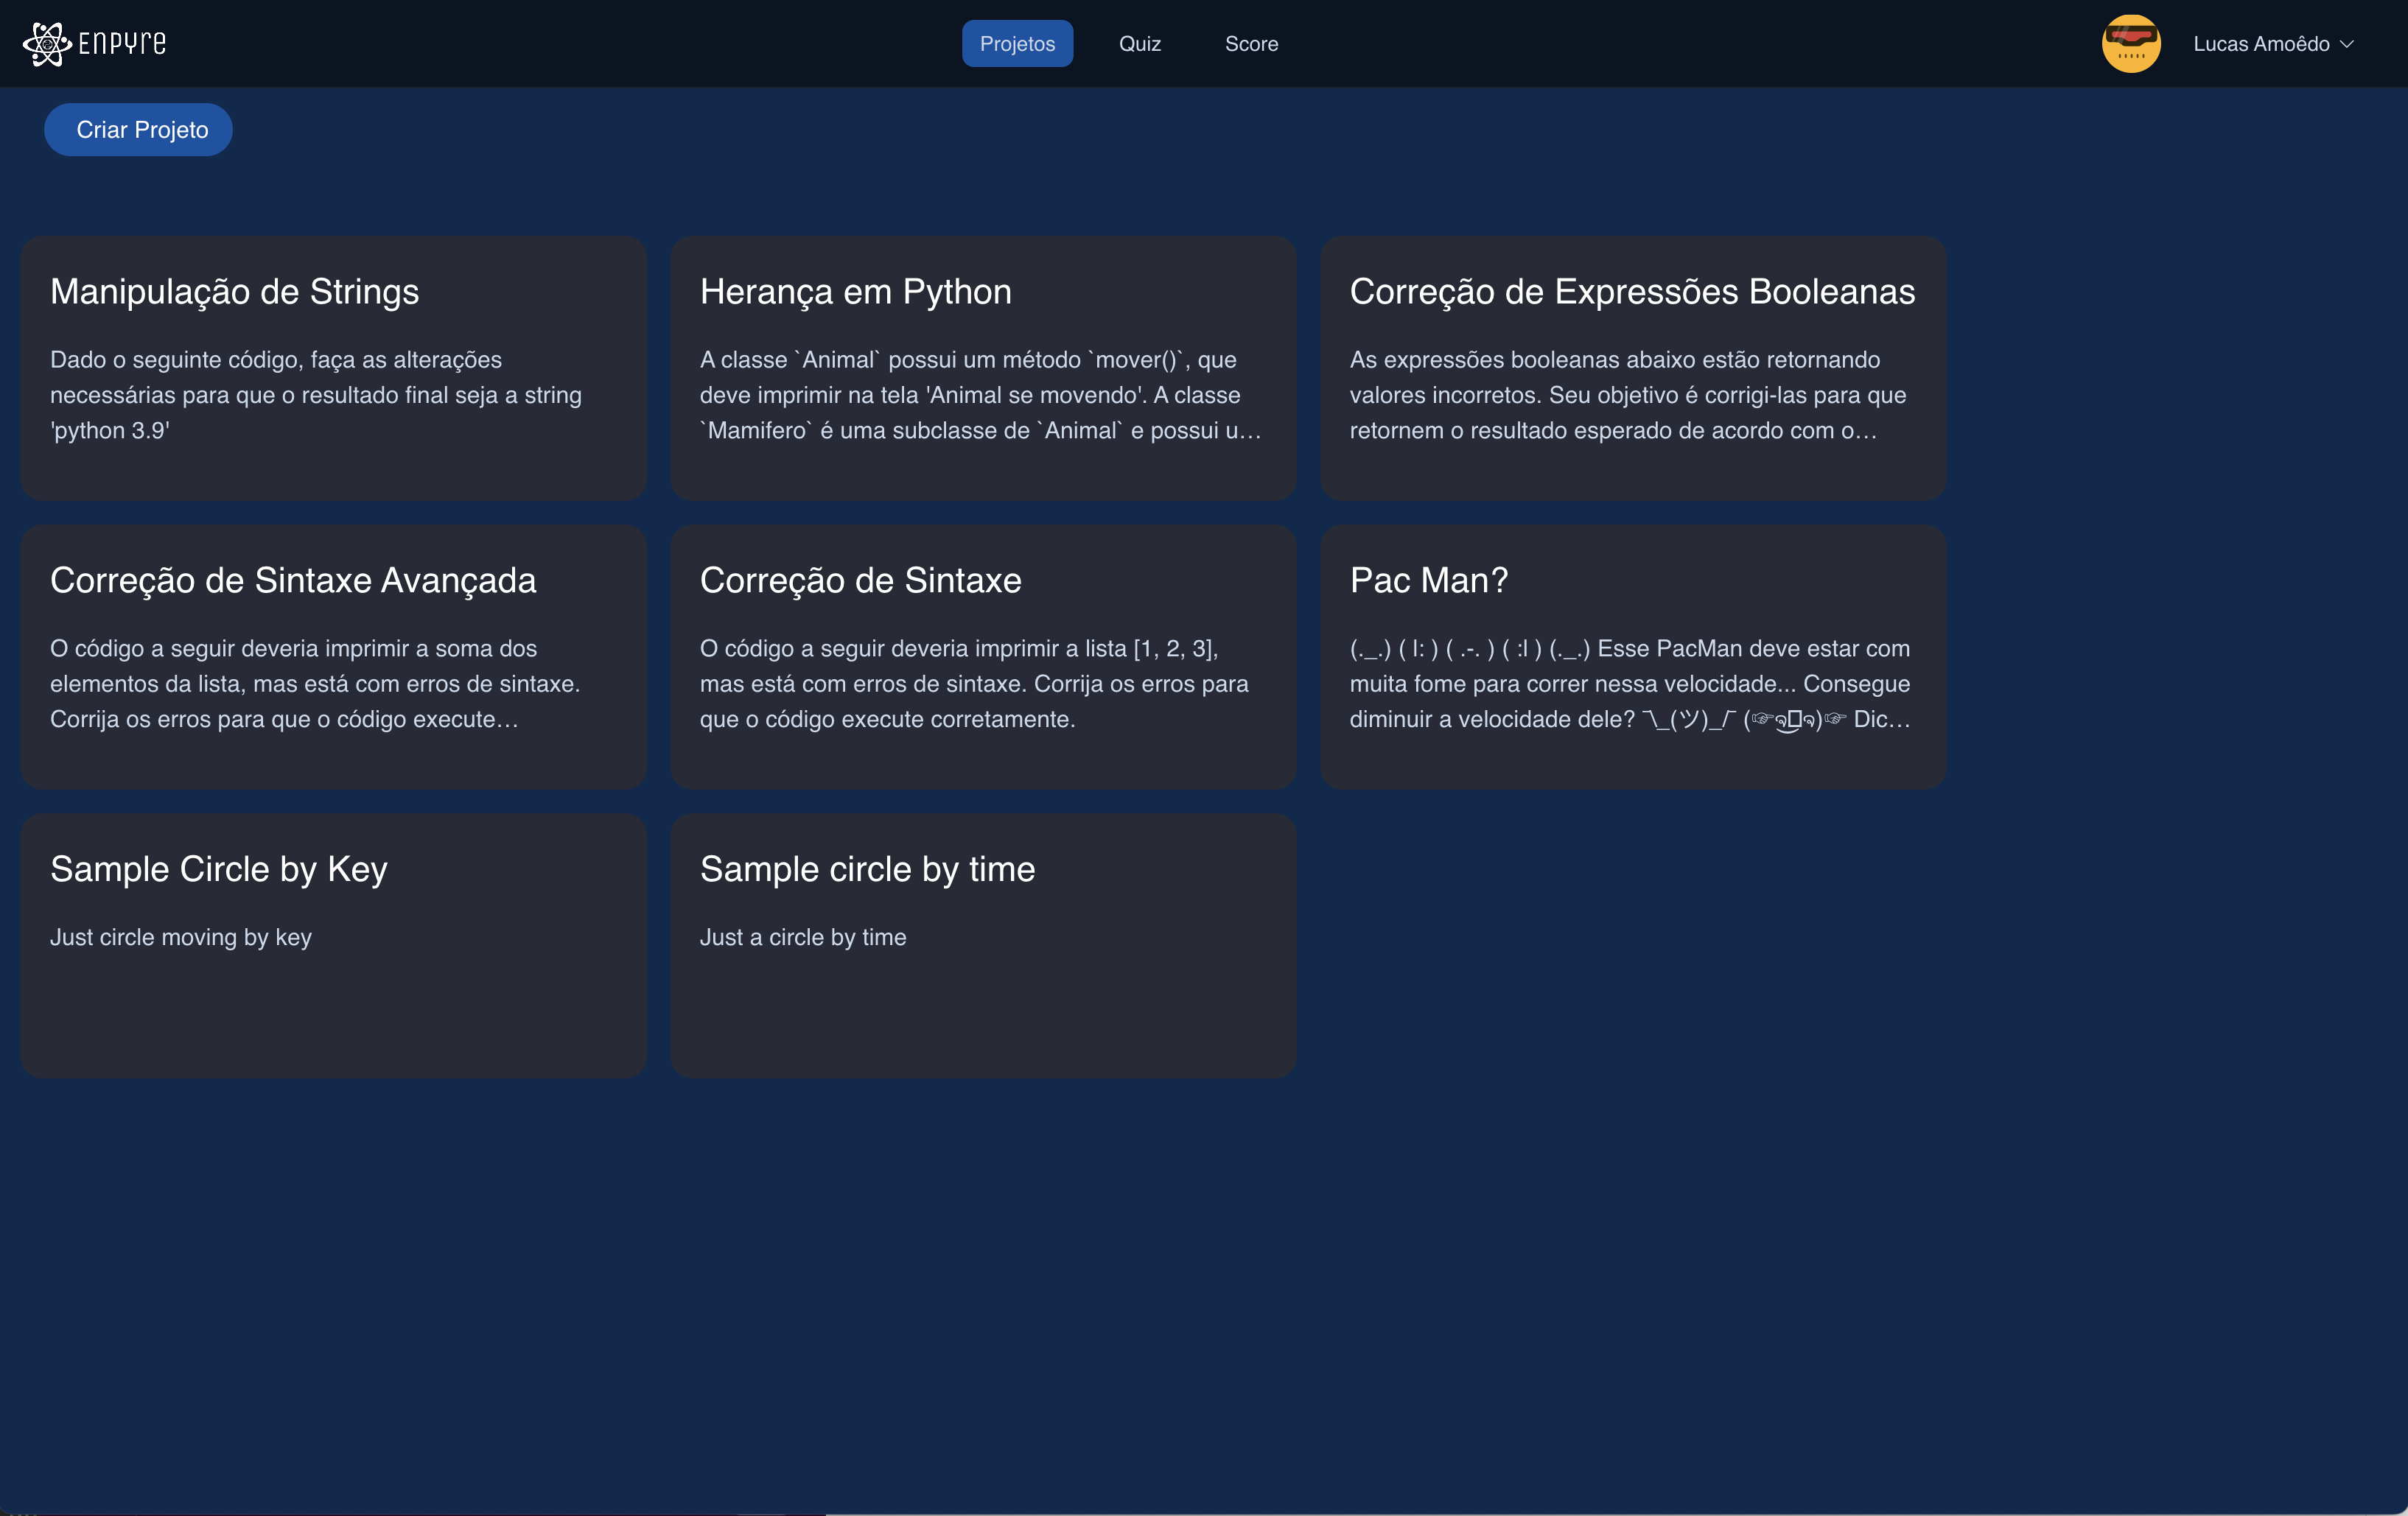
\includegraphics[width=0.8\textwidth]{figuras/projetos.eps}
    \caption{Tela de lista de projetos}
    \label{fig:lista-projetos}
\end{figure}

\begin{figure}[H]
    \centering
    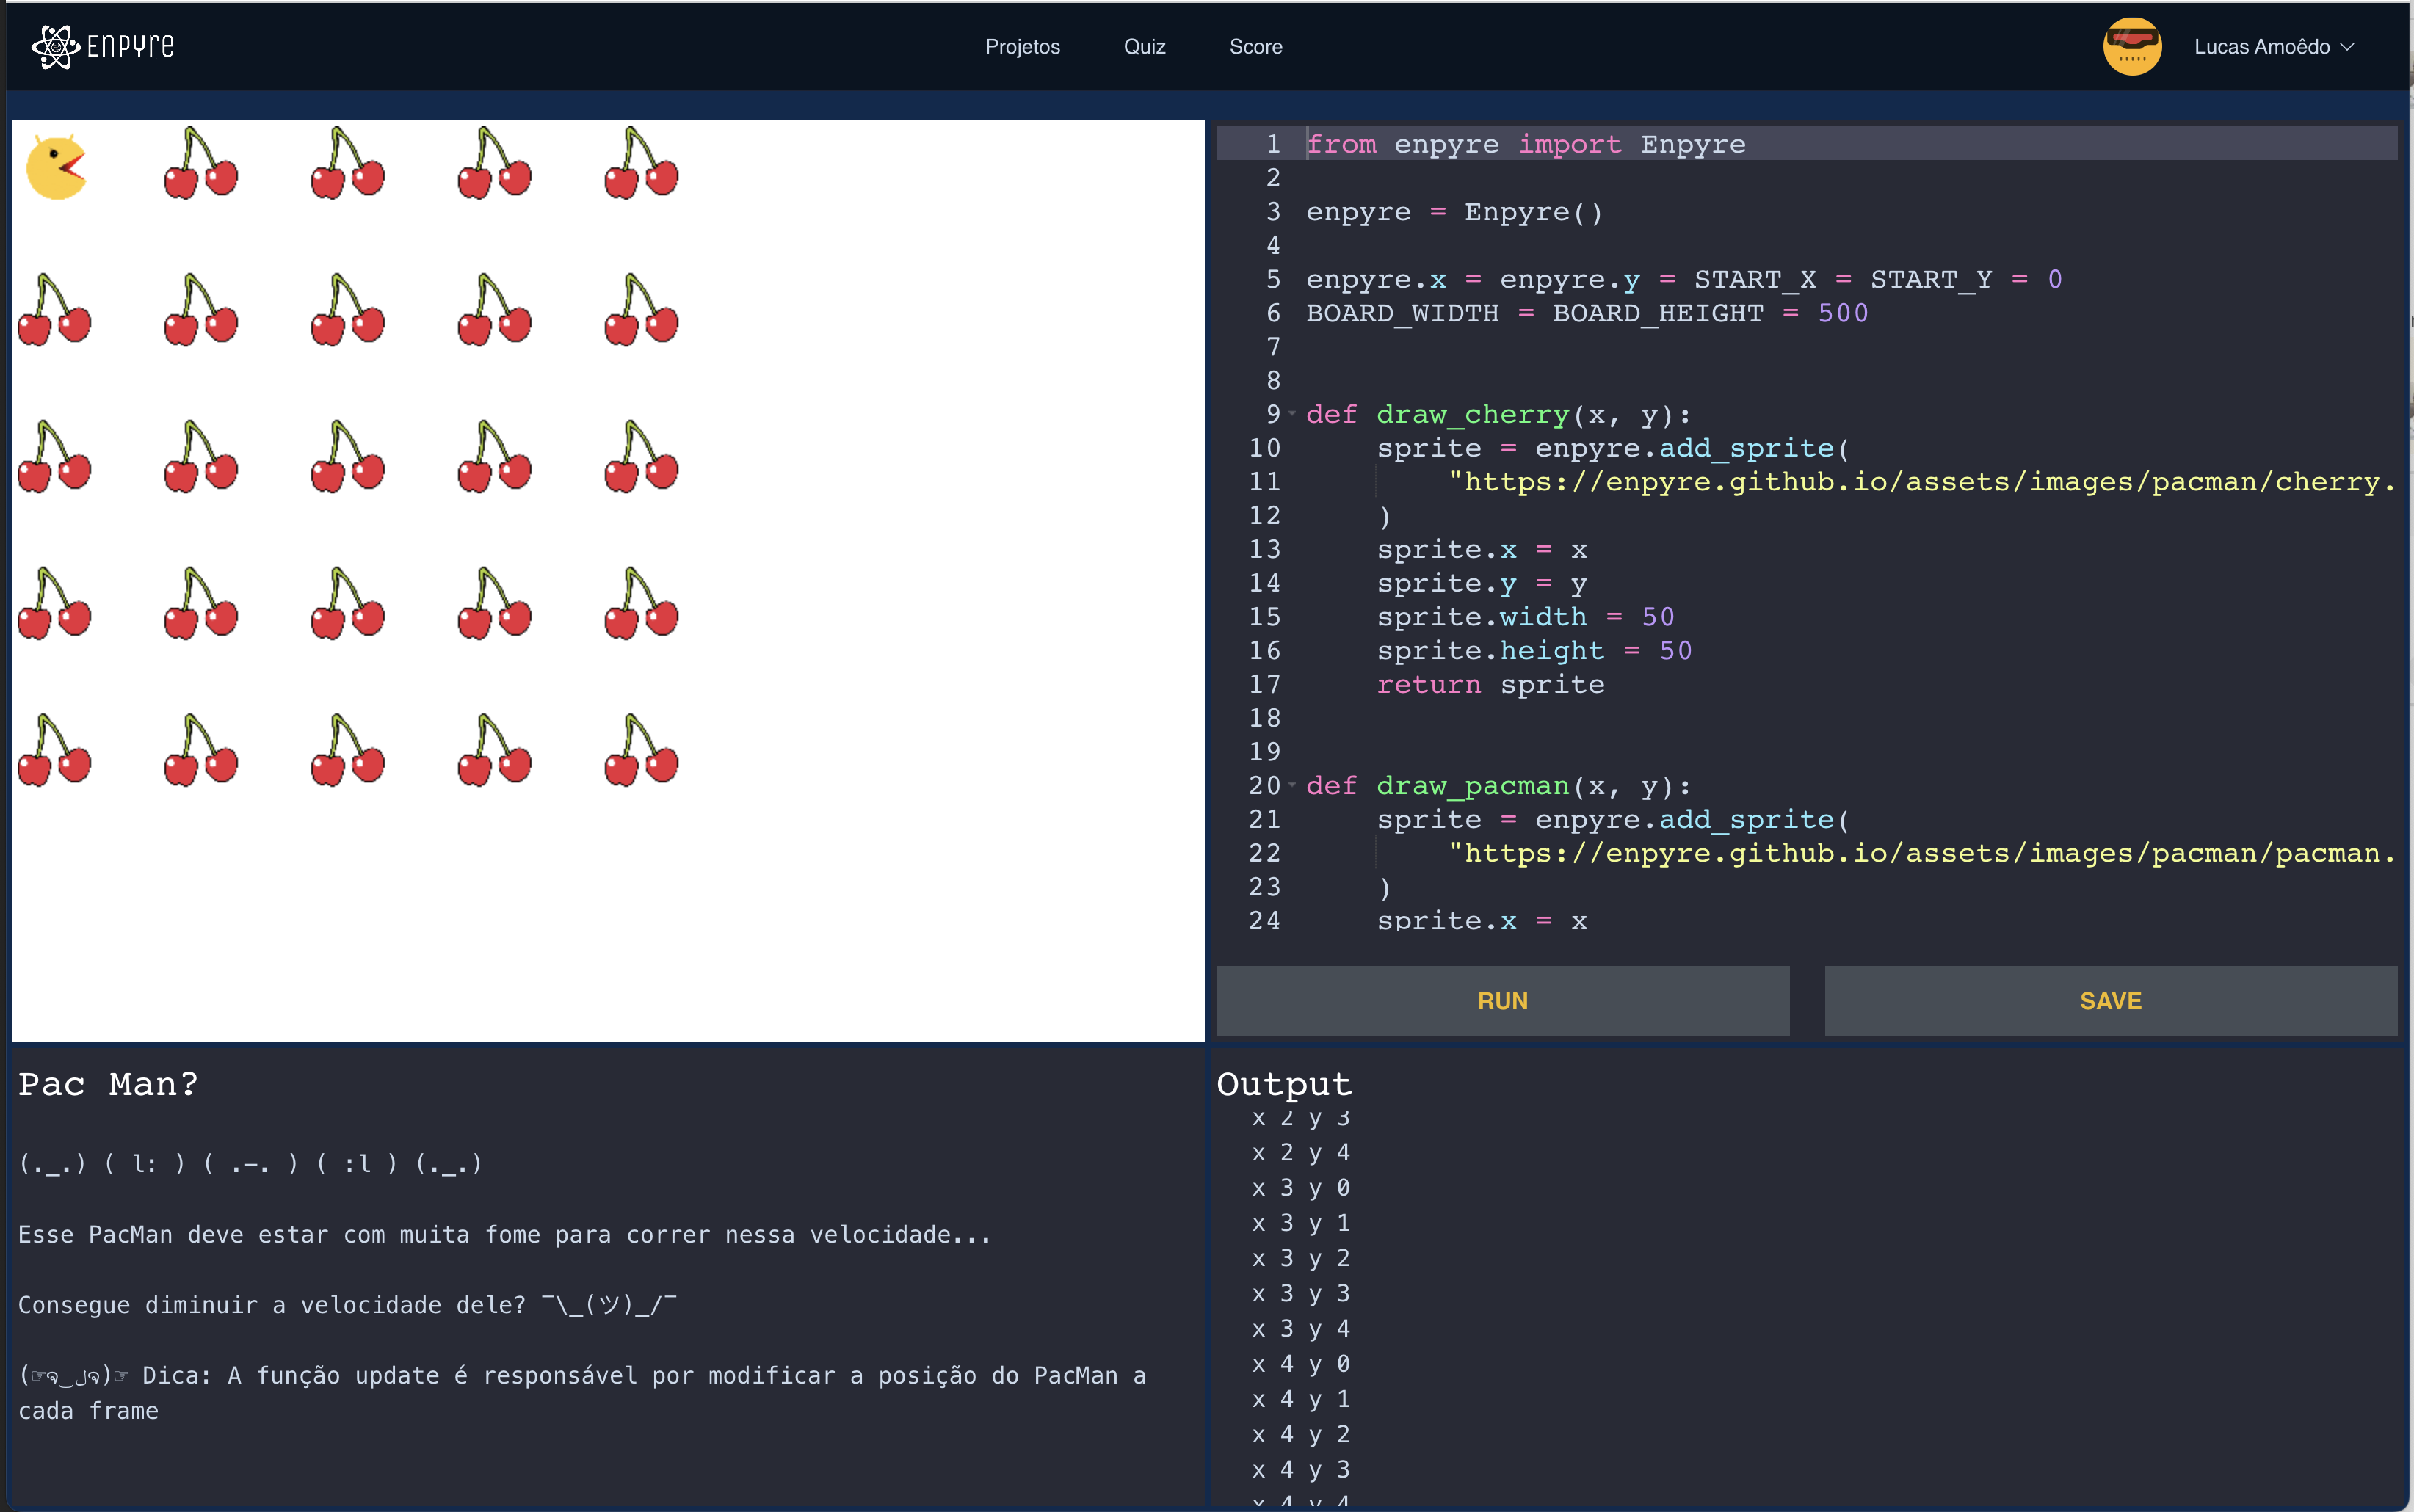
\includegraphics[width=0.8\textwidth]{figuras/projeto.eps}
    \caption{Tela do projeto}
    \label{fig:projeto}
\end{figure}

\subsection{Tela de quiz}

\begin{figure}[H]
    \centering
    \includegraphics[width=0.8\textwidth]{figuras/quizz_lista.eps}
    \caption{Tela de lista de quiz}
    \label{fig:quiz}
\end{figure}

\begin{figure}[H]
    \centering
    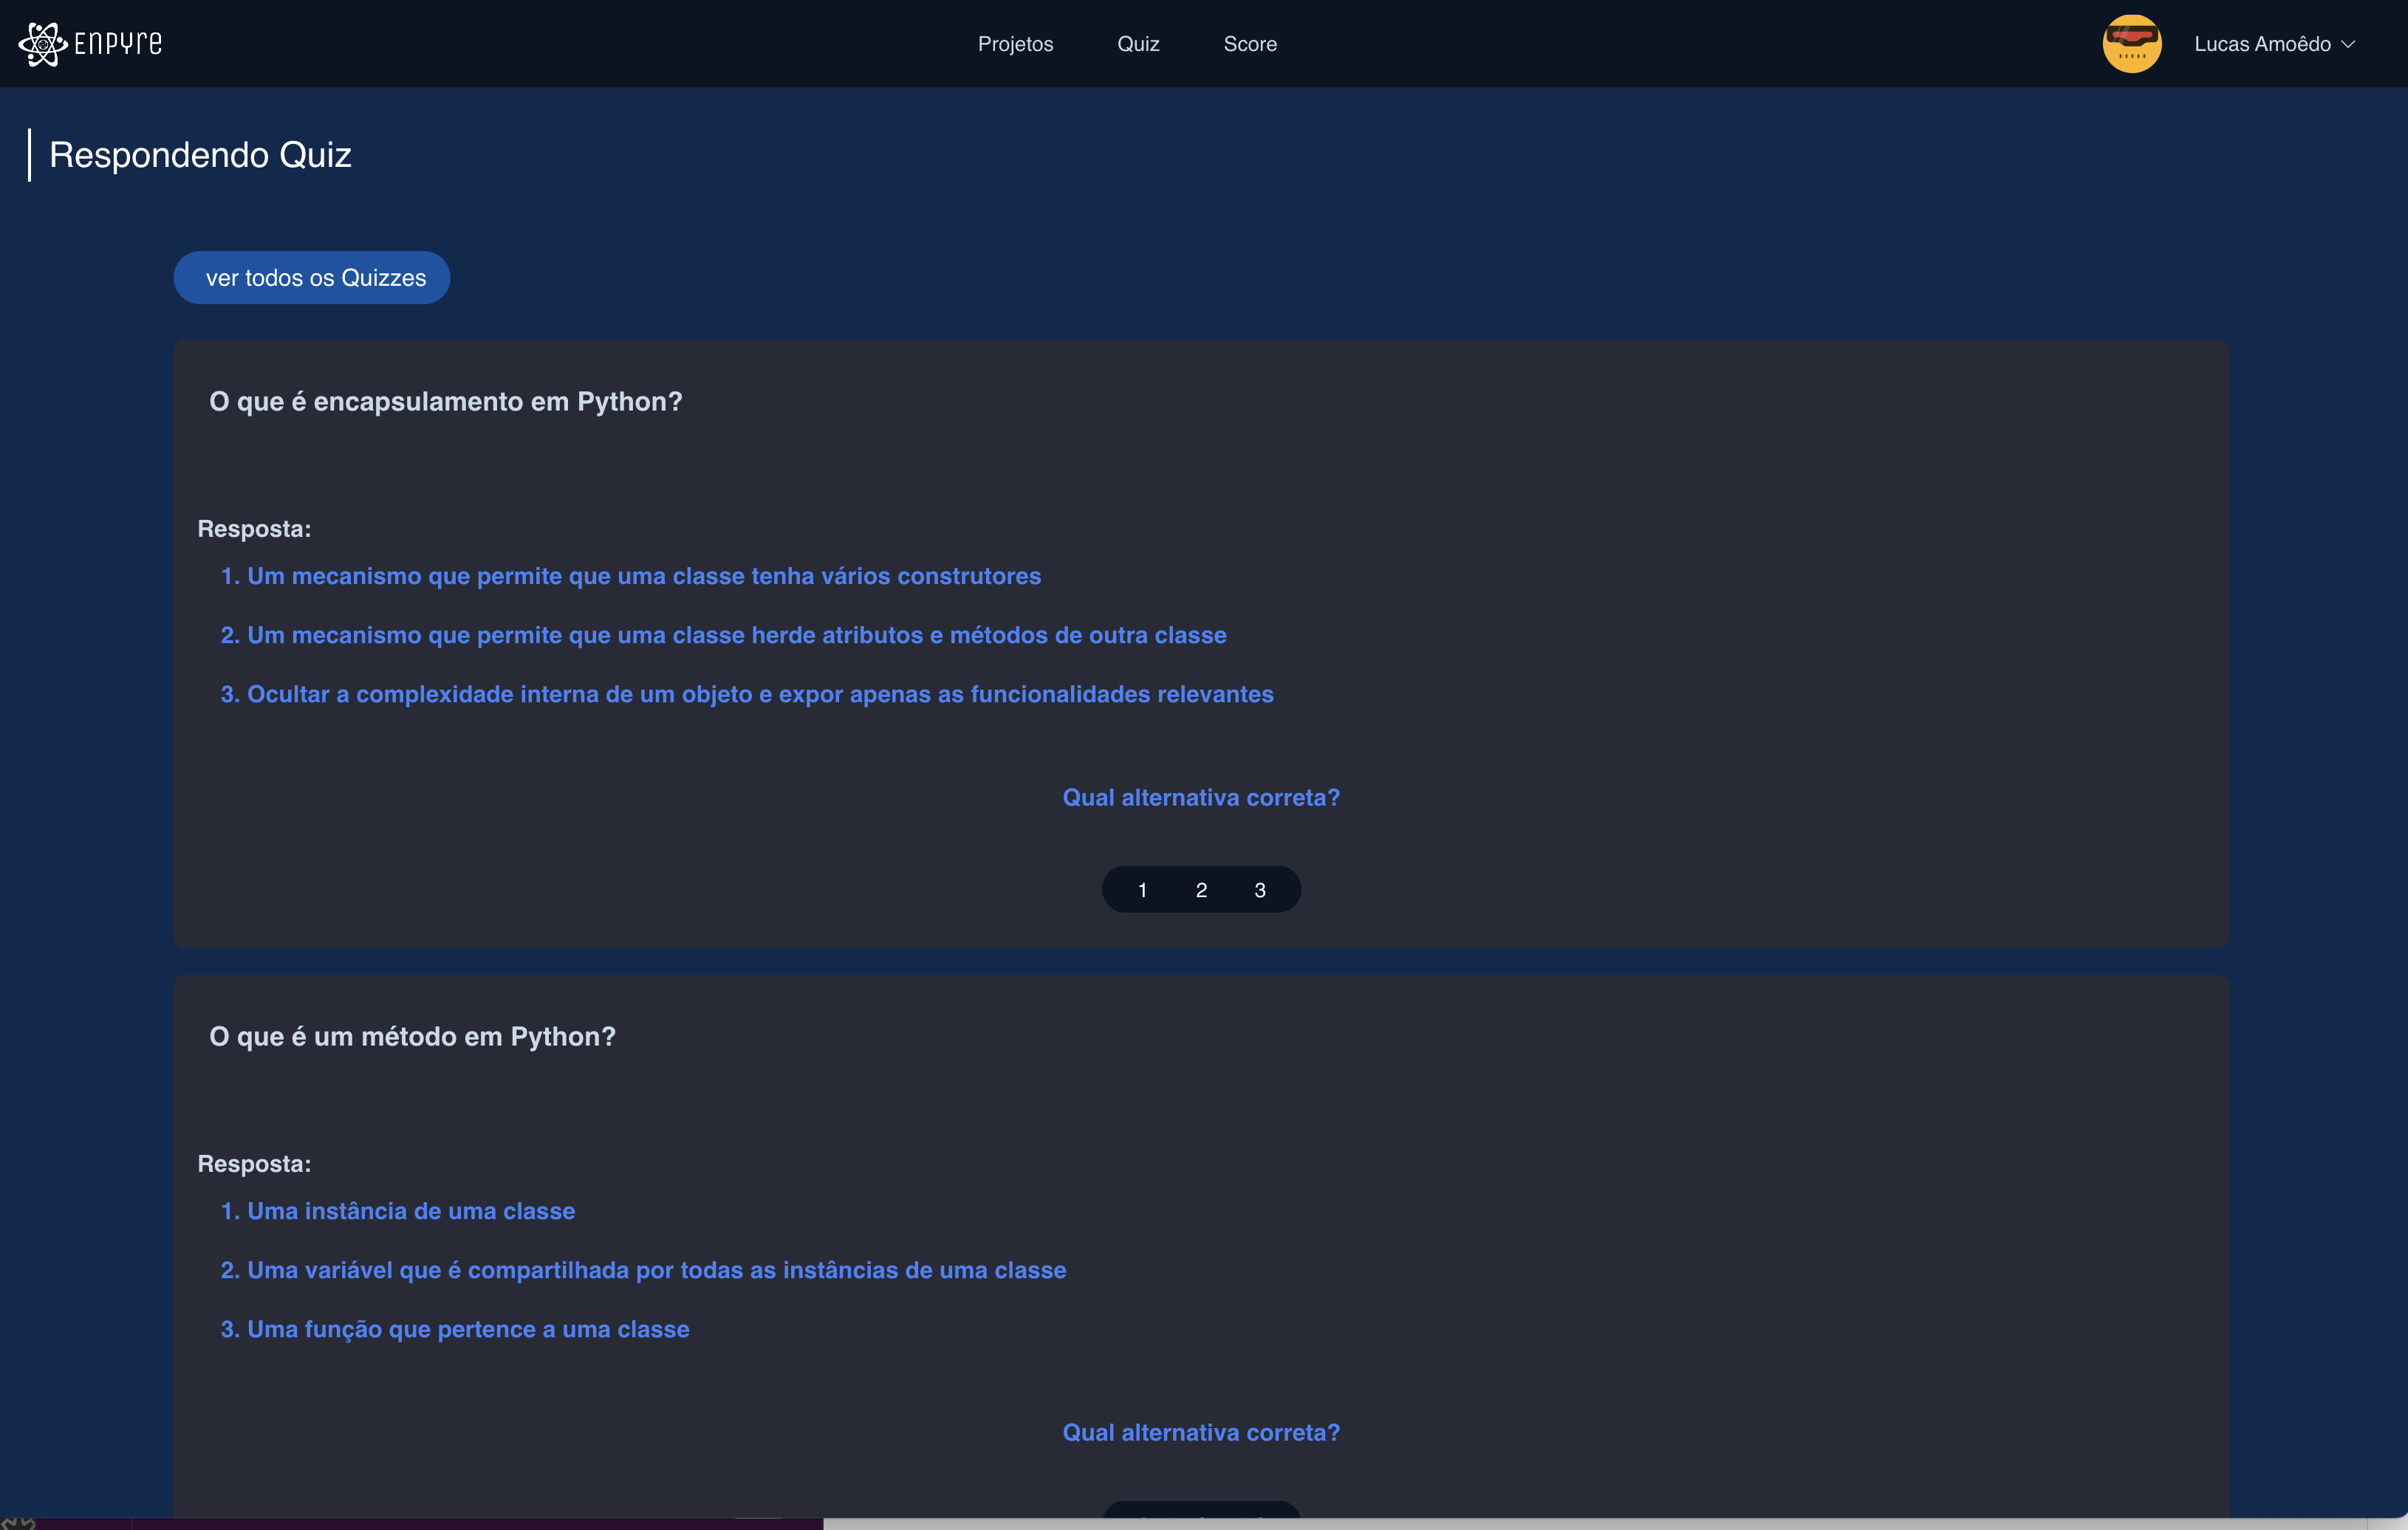
\includegraphics[width=0.8\textwidth]{figuras/quizz.eps}
    \caption{Tela do quiz}
    \label{fig:quiz}
\end{figure}

\section{Métricas de Qualidade}

Foi utilizado o \href{https://sonarcloud.io/projects}{SonarCloud} para realizar a análise estática de código e obter métricas de qualidade do código. As métricas finais obtidas podem ser vistas na imagem \ref{fig:sonarcloud}. A descrição das métricas de qualidade do código são apresentadas a seguir:

\begin{itemize}
    \item \textbf{\textit{Reliability}}: A métrica ``Reliability'' se refere à confiabilidade do código, ou seja, a capacidade do software em executar suas funcionalidades de forma consistente e livre de erros. Essa métrica avalia a estabilidade e robustez do código, medindo a probabilidade de ocorrência de falhas, erros de lógica, exceções não tratadas e comportamentos inesperados durante a execução do programa. É uma medida importante para garantir a qualidade do software, pois um código confiável é menos propenso a causar falhas e interrupções indesejadas.
    \item \textbf{\textit{Maintainability}}: A métrica ``Maintainability'' se refere à manutenibilidade do código, ou seja, a facilidade com que o código pode ser mantido, modificado e aprimorado ao longo do tempo. Essa métrica avalia a qualidade do código em termos de legibilidade, modularidade, organização e documentação. Um código com alta manutenibilidade é mais fácil de entender, depurar, estender e adaptar a novos requisitos ou correções. Isso é fundamental para permitir que equipes de desenvolvimento trabalhem de forma eficiente e reduzir o risco de introdução de erros durante as atividades de manutenção e evolução do software.
    \item \textbf{\textit{Security}}: A métrica ``Security'' se refere à segurança do código, ou seja, a capacidade do software em proteger dados sensíveis, prevenir vulnerabilidades e evitar ataques cibernéticos. Essa métrica avalia a robustez das medidas de segurança implementadas no código, como autenticação, autorização, criptografia e proteção contra ameaças conhecidas. Um código com alta segurança é menos suscetível a brechas de segurança e protege as informações confidenciais dos usuários e do sistema como um todo. Garantir a segurança do código é fundamental para evitar violações de segurança e proteger a integridade e privacidade dos dados.
    \item \textbf{\textit{Security Review}}: A ``Security Review'' é uma avaliação de segurança realizada no código ou em um sistema de software. Ela envolve a revisão minuciosa do código-fonte, infraestrutura e configurações de segurança para identificar possíveis vulnerabilidades, brechas ou falhas de segurança. Durante a revisão de segurança, são aplicadas técnicas e ferramentas específicas para analisar o código em busca de problemas de segurança conhecidos, padrões inseguros de programação e configurações inadequadas. O objetivo é identificar e corrigir quaisquer pontos fracos que possam ser explorados por hackers ou representar riscos à segurança do sistema.
    \item \textbf{\textit{Coverage}}: ``Coverage'' se refere à cobertura de código, uma métrica que mede a quantidade de código que foi exercitada por testes automatizados. Ela indica a porcentagem de linhas de código, ramificações condicionais ou funcionalidades que foram testadas pelo conjunto de testes. Quanto maior a cobertura, maior a confiança de que o código foi amplamente testado e que as diferentes partes do software estão funcionando corretamente. A cobertura de código é uma medida importante para avaliar a qualidade dos testes e a eficácia dos esforços de garantia de qualidade no desenvolvimento de software.
    \item \textbf{\textit{Duplications}}: ``Duplications'' se refere a duplicações de código, ou seja, trechos de código que aparecem repetidamente em diferentes partes do software. Essas duplicações podem ocorrer por várias razões, como falta de modularização, cópia e colagem excessiva de código, ou falta de reutilização de componentes. Identificar e analisar duplicações de código é importante para a manutenibilidade e qualidade do software, pois elas podem levar a problemas como dificuldade na manutenção, inconsistências, propagação de bugs e aumento da complexidade do código. Ao eliminar duplicações, é possível melhorar a legibilidade, eficiência e facilidade de manutenção do código.
\end{itemize}

\begin{figure}[H]
    \centering
    \includegraphics[width=1\textwidth]{figuras/sonarcloud.eps}
    \caption{Métricas de qualidade do código}
    \label{fig:sonarcloud}
\end{figure}
